%!TEX root = ./EpsilonBook.tex

\chapter{The Epsilon Generation Language (EGL)}
\label{sec:EGL}
EGL provides a language tailored for model-to-text transformation (M2T). EGL can be used to transform models into various types of textual artefact, including executable code (e.g. Java), reports (e.g. in HTML), images (e.g. using DOT), formal specifications (e.g. Z notation), or even entire applications comprising code in multiple languages (e.g. HTML, Javascript and CSS).

EGL is a \emph{template-based} code generator (i.e. EGL programs resemble the text that they generate), and provides several features that simplify and support the generation of text from models, including: a sophisticated and language-independent merging engine (for preserving hand-written sections of generated text), an extensible template system (for generating text to a variety of sources, such as a file on disk, a database server, or even as a response issued by a web server), formatting algorithms (for producing generated text that is well-formatted and hence readable), and traceability mechanisms (for linking generated text with source models). 

% TODO: improve merge engine section: running example and describe how to use protected regions in the generated text

% TODO Provide (one or more) table that summarises the operations available on out
% Note that the \verb|out| keyword also
% provides \emph{println(Object)} and \emph{chop(Integer)} methods, which
% can be used to construct text with linefeeds, and to remove the
% specified number of characters from the end of the generated text.

\section{Abstract Syntax}
Figure \ref{fig:abstractsyntax} depicts the abstract syntax of EGL's core functionality.

\begin{figure}[htbp]
  \begin{center}
    \leavevmode
    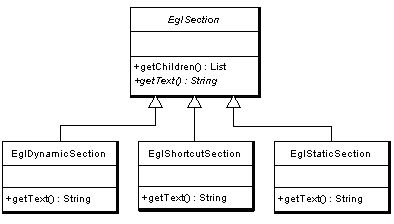
\includegraphics[scale=0.80]{images/EglAbstractSyntax.png}
  \end{center}
  \caption{The abstract syntax of EGL's core.}
  \label{fig:abstractsyntax}
\end{figure}

Conceptually, an EGL program comprises one or more \emph{sections}. The contents of static
sections are emitted verbatim and appear directly in the
generated text. The contents of dynamic sections are executed and are used
used to control the text that is generated.

In its dynamic sections, EGL re-uses EOL's mechanisms for structuring
program control flow, performing model inspection and navigation, and
defining custom operations. In addition, EGL provides an EOL object, \verb|out|,
which is used in dynamic sections to perform operations on the generated text, 
such as appending and removing strings; and specifying the type of text to be generated.

EGL also provides syntax for defining \textit{dynamic output}
sections, which provide a convenient shorthand for outputting text
from within dynamic sections. Similar syntax is often provided by
template-based code generators.

\section{Concrete Syntax}
\label{concretesyntax}

The concrete syntax of EGL closely resembles the style of other
template-based code generation languages, such as PHP. The tag pair \emph{[\% \%]} is
used to delimit a dynamic section. Any text not enclosed in such a tag
pair is contained in a static section. Listing
\ref{lst:basic} illustrates the use of dynamic and static sections to
form a basic EGL template.

\begin{lstlisting}[basicstyle=\ttfamily\footnotesize, language=EGL, tabsize=2, flexiblecolumns=true, caption=A basic EGL template., label=lst:basic]
[% for (i in Sequence{1..5}) { %]
i is [%=i%]
[% } %]
\end{lstlisting}

Executing the EGL template in Listing~\ref{lst:basic} would produce the generated
text in Listing~\ref{lst:basic-generated}. The \emph{[\%=expr\%]} construct (line 2) is shorthand for \emph{[\%
  out.print(expr); \%]}, which appends \emph{expr} to the output
generated by the transformation.

\begin{lstlisting}[basicstyle=\ttfamily\footnotesize, language=EGL, tabsize=2, flexiblecolumns=true, caption=The text generated from the basic EGL template (Listing~\ref{lst:basic})., label=lst:basic-generated]
i is 1
i is 2
i is 3
i is 4
i is 5
\end{lstlisting}

Any EOL statement can be contained in the dynamic sections of an EGL template.
For example, the EGL template depicted in Listing \ref{lst:oo} generates text
from a model that conforms to a metamodel that describes an
object-oriented system. % TODO include metamodel diagram

\begin{lstlisting}[basicstyle=\ttfamily\footnotesize, language=EGL, tabsize=2, flexiblecolumns=true, caption=Generating the name of each Class contained in an input model., label=lst:oo]
[% for (c in Class.all) { %]
[%=c.name%]
[% } %]
\end{lstlisting}

\subsection{User-Defined Operations}
Like EOL, EGL permits users to define re-usable units of code via operations (Section~\ref{sec:Design.EOL.Operations}). In EGL, user-defined operations  
are defined in dynamic sections, but may mix static and dynamic sections in their
bodies. Consider, for example, the EGL code in Listing~\ref{lst:egl_operation}, 
which emits a declaration for a Java class (e.g. \texttt{public class Foo \{\}}).
Lines 2-4 declare the operation. Note that the start and the end of the operation's 
declaration (on line 2 and 4, respectively) are contained in dynamic sections. The
body of the operation (line 3), however, mixes static and dynamic output sections.
Finally, note that the operation is invoked from a dynamic section (line 1).

\begin{lstlisting}[basicstyle=\ttfamily\footnotesize, language=EGL, tabsize=2, flexiblecolumns=true, caption=Using an operation to specify the text generated for a declaration of a Java class., label=lst:egl_operation]
[% c.declaration(); %]
[% operation Class declaration() { %]
[%=self.visibility] class [%=self.name%] {}
[% } %]
\end{lstlisting}

When a user-defined operation is invoked, any static or dynamic sections contained 
in the body of the operation are immediately appended to the generated text. Sometimes, 
however, it is desirable to manipulate the text produced by an operation before it is
appended to the generated text. To this end, EGL defines the \texttt{@template} annotation
which can applied to operations to indicate that any text generated by the operation
must be returned from the operation and not appended to the generated text. For example,
the EGL program in Listing~\ref{lst:egl_operation} could be rewritten using a \texttt{@template}
annotation, as demonstrated in Listing~\ref{lst:egl_template_operation}.

\begin{lstlisting}[float=tbp, basicstyle=\ttfamily\footnotesize, language=EGL, tabsize=2, flexiblecolumns=true, caption=Using a template operation to specify the text generated for a declaration of a Java class., label=lst:egl_template_operation]
[%=c.declaration()%]
[% @template
   operation Class declaration() { %]
[%=self.visibility] class [%=self.name%] {}
[% } %]
\end{lstlisting}

There is a subtle difference between the way in which standard (i.e. unannotated)
operations and \texttt{@template} operations are invoked. Compare the first line of Listings~\ref{lst:egl_operation} and~\ref{lst:egl_template_operation}. The former
uses a dynamic section, because invoking the operation causes the evaluation of 
its body to be appended to the text generated by this program. By contrast, the 
latter uses a dynamic output section to append the result returned by 
the \texttt{@template} operation to the text generated by this program.

In general, \texttt{@template} operations afford more flexibility than standard
operations. For example, line 1 of Listing~\ref{lst:egl_template_operation} could
perform some manipulation of the text returned by the \texttt{declaration()} operation
before the text is outputted. Therefore, \texttt{@template} operations provide
a mechanism for re-using common pieces of a code generator, without sacrificing the
flexibility to slightly alter text before it is emitted. Standard (unannotated) 
operations also permit re-use, but in a less flexible manner.

Finally, it is worth noting that user-defined operations in EGL do not have to 
generate text. For example, Listing~\ref{lst:egl_normal_operations} 
illustrates two operations defined in an EGL program that do not generate any text.
The former is a query that returns a Boolean value, while the latter alters the model,
and does not return a value.

\begin{lstlisting}[float=tbp, basicstyle=\ttfamily\footnotesize, language=EGL, tabsize=2, flexiblecolumns=true, caption=Operations that do not generate any text., label=lst:egl_normal_operations]
[%
  operation Class isAnonymous() : Boolean {
		return self.name.isUndefined();
  }

  operation removeOneClass() {
		delete Class.all.random();
	}
%]
\end{lstlisting}

\section{The OutputBuffer}
As an EGL program is executed, text is appended to a data structure termed 
the \emph{OutputBuffer}. In every EGL program, the \emph{OutputBuffer} is 
accessible via the \texttt{out} built-in variable. The \emph{OutputBuffer} 
provides operations for appending to and removing from the buffer, and for 
merging generated text with existing text (see Section~\ref{sec:merging}).

For many EGL programs, interacting directly with the \emph{OutputBuffer} is 
unnecessary. The contents of static and dynamic output sections are sent 
directly to the \emph{OutputBuffer}, and no operation of the \emph{OutputBuffer}
need be invoked directly. However, in cases when generated text must be sent
to the \emph{OutputBuffer} from dynamic sections, or when generated text must
be merged with existing text, the operations of \emph{OutputBuffer} (Table~\ref{tab:OutputBufferOperations}) are provided. Section~\ref{sec:merging}
discusses merging generated and existing text, and presents several examples
of invoking the operations of \emph{OutputBuffer}.

\begin{longtable} {|p{5.5cm}|p{6.5cm}|}
			
			\caption{Operations of type Template}
			\label{tab:OutputBufferOperations}\\
			
			\hline
							
			\textbf{Signature} & \textbf{Description} \\\hline
			
			chop(numberOfChars : Integer) & Removes the specified number of characters from the end of the buffer \\\hline
			
			print(object : Any) & Appends a string representation of the specified object to the buffer \\\hline
			
			println(object : Any) & Appends a string representation of the specified character and a new line to the buffer \\\hline
			
			println() & Appends a new line to the buffer \\\hline
			
			setContentType(contentType : String) & Updates the content type of this template. Subsequent calls to \texttt{pr\-es\-er\-ve} or \texttt{st\-a\-rtPr\-es\-er\-ve} that do not specify a style of comment will use the style of comment defined by the specified content type. See Section~\ref{sec:merging}. \\\hline
			
			preserve(id : String, enabled : Boolean, contents : String) & Appends a protected region to the buffer with the given identifier, enabled state and contents. Uses the current content type to determine how to format the start and end markers. See Section~\ref{sec:merging}. \\\hline
			
			preserve(startComment : String, endComment : String, id : String, enabled : Boolean, contents : String) & Appends a protected region to the buffer with the given identifier, enabled state and contents. Uses the first two parameters as start and end markers. See Section~\ref{sec:merging}. \\\hline
			
			startPreserve(id : String, enabled : Boolean) & Begins a protected region by appending the start marker for a protected region to the buffer with the given identifier and enabled state. Uses the current content type to determine how to format the start and end markers. See Section~\ref{sec:merging}. \\\hline
			
			startPreserve(startComment : String, endComment : String, id : String, enabled : Boolean) & Begins a protected region by appending the start marker to the buffer with the given identifier and enabled state. Uses the first two parameters as start and end markers. See Section~\ref{sec:merging}. \\\hline
			
			stopPreserve() & Ends the current protected region by appending the end marker to the buffer. This operation should be invoked only if there a protected region is currently open (i.e. has been started by invoking \texttt{st\-a\-rtPr\-es\-er\-ve} but not yet stopped by invoking \texttt{st\-opPr\-es\-er\-ve}). See Section~\ref{sec:merging}. \\\hline
\end{longtable}

\section{Co-ordination}
\label{Co-ordination}
In the large, M2T transformations are used to generate text to various
destinations. For example, code generators often produce files on disk, 
and web applications often generate text as part of the response for a 
resource on the web server. Text might be generated to a network socket
during interprocess communication, or as a query that runs on a database.
Furthermore, (parts of) a single M2T transformation might be re-used in 
different contexts. A M2T transformation that generates files on disk today 
might be re-purposed to generate the response from a web server tomorrow.  

Given these concerns, EGL provides a co-ordination engine that provides
mechanisms for modularising M2T transformations, and for controlling the
destinations to which text is generated. The EGL co-ordination engine 
fulfils three requirements:

\begin{enumerate}
	\item \textbf{Reusability}: the co-ordination engine allows EGL programs to be
	                   decomposed into one or more templates, which
	                   can be shared between EGL programs.

	\item \textbf{Variety of destination}: the co-ordination engine provides an
	                              extensible set of template types that can
	                              generate text to a variety of destinations.
	                              Section~\ref{sec:egl_template_type} describes
	                              the default template type, which is 
	                              tailored to generate text to files on disk, 
	                              while Section~\ref{sec:custom_co-ordination} 
	                              discusses the way in  which users can define 
	                              their own template types for generating text to
	                              other types of destination.
	
	\item \textbf{Separation of concerns}: the co-ordination engine ensures that the 
	                              logic for controlling the text that is
	                              generated (i.e. the content) and the logic for
	                              controlling the way in which text is emitted
	                              (i.e. the destination) are kept separate.
\end{enumerate}

\subsection{The Template type}
\label{sec:egl_template_type}
Central to the co-ordination engine is the \emph{Template} type, 
which EGL provides in addition to the default EOL types
(Section~\ref{sec:eol_types}). Via the \emph{Template} type, EGL
fulfils the three requirements identified above. Firstly, a \emph{Template} 
can invoke other \emph{Templates}, and hence can be shared and re-used 
between EGL programs. Secondly, the \emph{Template} type has been implemented
in an extensible manner: users can define their own types of \emph{Template} 
that generate text to any destination (e.g. a database or a network
socket), as described in Section~\ref{sec:custom_co-ordination}. Finally, 
the \emph{Template} type provides a set of operations that are used to 
control the destination of generated text. Users typically define a ``driver''
template that does not generate text, but rather controls the destination 
of text that is generated by other templates. 

For example, consider the EGL program in Listing~\ref{lst:co-ordination}.
This template generates no text (as it contains only a single dynamic section),
but is used instead to control the destination of text generated by another
template. Line 1 defines a variable, \texttt{t}, of type \emph{Template}. 
Note that, unlike the EOL types, instances of \emph{Template} are not created
with the \texttt{new} keyword. Instead, the \emph{TemplateFactory} built-in
object (Section~\ref{sec:template_factory}) is used to load templates from, 
for example, a file system path. On line 3, the \emph{generate} operation 
of the \emph{Template} type invokes the EGL template
stored in the file ``ClassNames.egl'' and emits the generated text to 
``Output.txt''.

\begin{lstlisting}[basicstyle=\ttfamily\footnotesize, language=EGL, tabsize=2, flexiblecolumns=true, caption=Storing the name of each Class to disk., label=lst:co-ordination]
[%
  var t : Template = TemplateFactory.load("ClassNames.egl");
  t.generate("Output.txt");
%]
\end{lstlisting}

In addition to \texttt{generate}, the Template type defines further operations for controlling the context and invocation of EGL templates. Table~\ref{tab:TemplateOperations} lists all of the operations defined on \emph{Template}, and a further example of their use is given in Section~\ref{sec:example_of_co-ordination}.

\begin{longtable} {|p{5.5cm}|p{6.5cm}|}
			
			\caption{Operations of type Template}
			\label{tab:TemplateOperations}\\
			
			\hline
							
			\textbf{Signature} & \textbf{Description} \\\hline
			
			populate(name : String, value : Any) & Makes a variable with the specified name and value available during the execution of the template. \\\hline
			
			process() : String & Executes the template and returns the text that is generated.  \\\hline
			
			generate(destination : String) & Executes the template and stores the text to the specified destination. The format of the destination parameter is dictated by the type of template. For example, the default template type (which can generate files on disk) expects a file system path as the destination parameter. \\\hline
			
			setFormatter(formatter : Formatter) & Changes the formatter for this template to the specified formatter. Subsequent calls to generate or process will produce text that is formatted with the specified formatter. See Section~\ref{sec:formatters}. \\\hline
			
			setFormatters(formatters : Sequence(Formatter)) & Changes the formatter for this template to the specified sequence of formatters. Subsequent calls to generate or process will produce text that is formatted with each of the specified formatters in turn. See Section~\ref{sec:formatters}. \\\hline
\end{longtable}


\subsection{The TemplateFactory object}
As discussed above, instances of \emph{Template} are not created with the \texttt{new} keyword. Instead, EGL provides a built-in object, the \emph{TemplateFactory}, for this purpose. Users can customise the type of the \emph{TemplateFactory} object to gain more control over the way in which text is generated (Section~\ref{sec:custom_co-ordination}).

By default, EGL provides a \emph{TemplateFactory} that exposes operations for loading templates (by loading files from disk), preparing templates (by parsing a string containing EGL code), and for controlling the file system locations from which templates are loaded and to which text is generated. Table~\ref{tab:TemplateFactoryOperations} lists the operations provided by the built-in \emph{TemplateFactory} object. 

\label{sec:template_factory}
\begin{longtable} {|p{5.5cm}|p{6.5cm}|}
			
			\caption{Operations of the TemplateFactory object}
			\label{tab:TemplateFactoryOperations}\\
			
			\hline
							
			\textbf{Signature} & \textbf{Description} \\\hline
			
			load(path : String) : Template & Returns an instance of \emph{Template} that can be used to execute the EGL template stored at the specified path.  \\\hline
			
			prepare(code : String) : Template & Returns an instance of \emph{Template} that can be used to execute the specified EGL code.  \\\hline
			
			setRoot(path : String) & Changes the default path that is used to resolve relative paths when generating files to disk. Subsequent calls to load and prepare will create templates that use the new path. \\\hline
			
			setTemplateRoot(path : String) & Changes the default path that is used to resolve relative paths when loading templates with the load operation. Subsequent calls to load will use the new path. \\\hline
			
			setDefaultFormatter(formatter : Formatter) & Changes the formatter for this template factory to the specified formatter. Templates that are constructed after this
operation has been invoked will produce text that is, by default, formatted with the specified formatter. See Section~\ref{sec:formatters}. \\\hline
			
			setDefaultFormatters(fo\-rm\-at\-te\-rs : Sequence(Formatter)) & Changes the formatter for this template to the specified sequence of formatters. Templates that are constructed after this operation has been invoked will produce text that is, by default, formatted with each of the specified formatters in turn. See Section~\ref{sec:formatters}.  \\\hline
\end{longtable}

\subsection{An Example of Co-ordination with EGL}
\label{sec:example_of_co-ordination}
The operations provided by the \emph{TemplateFactory} object and \emph{Template} type are demonstrated by the EGL program in Listing~\ref{lst:co-ordination_complete}. Lines 2-3 use operations on \emph{TemplateFactory} to change the paths from which templates will be loaded (line 2) and to which generated files will be created (line 3). Line 5 demonstrates the use of the \texttt{prepare} operation for creating a template from EGL code. When the \texttt{interface} template is invoked, the EGL code passed to the \texttt{prepare} operation will be executed. Finally, line 9 (and line 12) illustrates the way in which the \texttt{populate} operation can be used to pass a value to a template before invoking it. Specifically, the interface and implementation templates can use a variable called \emph{root}, which is populated by the driver template before invoking them.

\begin{lstlisting}[basicstyle=\ttfamily\footnotesize, language=EGL, tabsize=2, flexiblecolumns=true, caption=Using the various operations provided by the Template type and TemplateFactory object., label=lst:co-ordination_complete]
[%
  TemplateFactory.setTemplateRoot("/usr/franz/templates");
	TemplateFactory.setRoot("/tmp/output");

  var interface      : Template =
    TemplateFactory.prepare("public interface [%=root.name] {}");
	
	var implementation : Template = 
	  TemplateFactory.load("Class2Impl.egl");

	for (c in Class.all) {
	  interface.populate("root", c);	
  	interface.generate("I" + c.name + ".java");
		
		implementation.populate("root", c);
		implementation.generate(c.name + ".java");
	}
%]
\end{lstlisting}

\subsection{Customising the Co-ordination Engine}
\label{sec:custom_co-ordination}
EGL provides mechanisms for customising the co-ordination engine. Specifically,
users can define and use their own \emph{TemplateFactory}. In many cases, 
users need not customise the co-ordination engine, and can write transformations
using the built-in \emph{Template} type and \emph{TemplateFactory} object. If, 
however, you need more control over the co-ordination process, the discussion in
this section might be helpful. Specifically, a custom \emph{TemplateFactory} 
is typically used to achieve one or more of the following goals:


\begin{enumerate}
	\item Provide additional mechanisms for constructing \emph{Templates}. 
	      \textbf{Example:} facilitate the loading of templates from a database.
	\item Enrich / change the behaviour of the built-in \emph{Template} type.
	      \textbf{Example:} change the way in which generated text is sent to its destination.
	\item Observe or instrument the transformation process by, for instance, logging calls to
	      the operations provided by the \emph{Template} type of the \emph{TemplateFactory}
	      object.
	      \textbf{Example:} audit or trace the transformation process.
\end{enumerate}

Customisation is achieved in two stages: implementing the custom \emph{TemplateFactory} 
(and potentially a custom \emph{Template}) in Java, and using the custom 
\emph{TemplateFactory}. 

\subsubsection{Implementing a custom TemplateFactory}
A custom \emph{TemplateFactory} is a subclass of \texttt{EglTemplateFactory}. Typically, 
a custom \emph{TemplateFactory} is implemented by overriding one of the methods of 
\texttt{EglTemplateFactory}. For example, the \texttt{createTemplate} method is 
overriden to specify that a custom type of \emph{Template} should be created by the \emph{TemplateFactory}. Likewise, the \texttt{load} and \texttt{prepare} methods can
be overriden to change the location from which \emph{Template}s are constructed.

A custom \emph{Template} is a subclass of \texttt{EglTemplate} or, most often, a 
subclass of \texttt{EglPersistentTemplate}. Again, customisation is typically 
achieved by overriding methods in the superclass, or by adding new methods. For 
example, to perform auditing activities whenever a template is used to generate
text, the \texttt{doGenerate} method of \texttt{EglPersistentTemplate} is
overriden.


\begin{lstlisting}[basicstyle=\ttfamily\footnotesize, language=Java, tabsize=2, flexiblecolumns=true, caption=A simple customisation of the co-ordination engine to count the number of calls to \texttt{generate()}., label=lst:custom_co-ordination_example]
import org.eclipse.epsilon.egl.EglFileGeneratingTemplateFactory;
import org.eclipse.epsilon.egl.EglTemplate;
import org.eclipse.epsilon.egl.EglPersistentTemplate;
import org.eclipse.epsilon.egl.exceptions.EglRuntimeException;
import org.eclipse.epsilon.egl.execute.context.IEglContext;
import org.eclipse.epsilon.egl.spec.EglTemplateSpecification;

public class CountingTemplateFactory 
extends EglFileGeneratingTemplateFactory {

	@Override
	protected EglTemplate createTemplate(EglTemplateSpecification spec) 
	throws Exception {
		return new CountingTemplate(spec,
		                            context,
		                            getOutputRootOrRoot(),
		                            outputRootPath);
	}	

  public class CountingTemplate 
  extends EglPersistentTemplate {

		public static int numberOfCallsToGenerate = 0;

		public CountingTemplate(EglTemplateSpecification spec,
		                        IEglContext context,
		                        URI outputRoot,
		                        String outputRootPath)
		throws Exception {
			super(spec, context, outputRoot, outputRootPath);
		}



		@Override
		protected void doGenerate(File file,
			                        String targetName,
			                        boolean overwrite,
			                        boolean protectRegions) 
		throws EglRuntimeException {
			numberOfCallsToGenerate++;
		}
	}
}
\end{lstlisting}

\subsubsection{Using a custom TemplateFactory}
When invoking an EGL program, the user may select a custom \emph{TemplateFactory}.
For example, the EGL development tools provide an Eclipse launch configuration that 
provides a tab named ``Generated Text.'' On this tab, users can select a 
\emph{TemplateFactory} (under the group called ``Type of Template Factory''). 
Note that a \emph{TemplateFactory} only appears on the launch configuration tab 
if it has been registered with EGL via an Eclipse extension. Similarly, the workflow language provided by Epsilon (Chapter~\ref{chp:Workflow}) allows the
specification of custom types of \emph{TemplateFactory} via the \texttt{te\-m\-pl\-a\-teFa\-ct\-o\-ryTy\-pe} parameter.


\subsection{Summary}
The co-ordination engine provided by EGL facilitates the construction
of modular and re-usable M2T transformations and can be used to generate 
text to various types of destination. Furthermore, the logic for 
specifying the contents of generated text is kept separate 
from the logic for specifying the destination of generated text.

\section{Merge Engine}
\label{sec:merging}
EGL provides language constructs that allow M2T transformations to
designate regions of generated text as \textit{protected}. Whenever 
an EGL program attempts to generate text, any protected regions that
are encountered in the specified destination are preserved.

Within an EGL program, protected regions are specified with the \emph{preserve(String, String,
  String, Boolean, String)} method on the \verb|out| keyword. The first two parameters define the comment delimiters of the target language. The other parameters provide the name,
enable-state and content of the protected region, as
illustrated in Listing \ref{lst:preserve}. 

\begin{lstlisting}[basicstyle=\ttfamily\footnotesize, language=EGL, tabsize=2, flexiblecolumns=true, caption=Protected region declaration using the preserve method., label=lst:preserve]
[%=out.preserve("/*", "*/", "anId", true,
                "System.out.println(foo);")
%]
\end{lstlisting}

A protected region declaration may have many lines, and use many EGL
variables in the contents definition.  To enhance readability, EGL
provides two additional methods on the \verb|out| keyword:
\emph{startPreserve(String, String, String, Boolean)} and
\verb|stopPreserve|.  Listing \ref{lst:startpreserve} uses these to
generate a protected region equivalent to that in Listing
\ref{lst:preserve}.

\begin{lstlisting}[basicstyle=\ttfamily\footnotesize, language=EGL, tabsize=2, flexiblecolumns=true, caption=Protected region declaration., label=lst:startpreserve]
[%=out.startPreserve("/*", "*/", "anId", true)%]
System.out.println(foo);
[%=out.stopPreserve()%]
\end{lstlisting}

Because an EGL template may contain many protected regions, EGL also
provides a separate method to set the target language generated by the
current template, \emph{setContentType(String)}. By default, EGL recognises Java, HTML, 
Perl and EGL as valid content types. An alternative configuration file
can be used to specify further content
types. Following a call to \verb|setContentType|, the first two
arguments to the \verb|preserve| and \verb|startPreserve| methods can
be omitted, as shown in Listing \ref{lst:contenttype}.

\begin{lstlisting}[basicstyle=\ttfamily\footnotesize, language=EGL, tabsize=2, flexiblecolumns=true, caption=Setting the content type., label=lst:contenttype]
[% out.setContentType("Java"); %]
[%=out.preserve("anId", true, "System.out.println(foo);")%]
\end{lstlisting}

Because some languages define more than one style of comment
delimiter, EGL allows mixed use of  the styles for \verb|preserve| and
\verb|startPreserve| methods.

Once a content type has been specified, a protected region may also be declared entirely from a static section, using the syntax in Listing \ref{lst:manualpr}.

\begin{lstlisting}[basicstyle=\ttfamily\footnotesize, language=EGL, tabsize=2, flexiblecolumns=true, caption=Declaring a protected region from within a static section., label=lst:manualpr]
[% out.setContentType("Java"); %]
// protected region anId [on|off] begin
System.out.println(foo);
// protected region anId end
\end{lstlisting}

When a template that defines one or more protected regions is
processed by the EGL execution engine, the target output destinations
are examined and existing contents of any protected regions are
preserved. If either the output generated by from the template or the
existing contents of the target output destination contains protected
regions, a merging process is invoked. Table \ref{tab:merging} shows
the default behaviour of EGL's merge engine.

\begin{table}[htbp]
  \begin{center}
  \begin{tabular}{|l|l|l|}
  \hline
  \multicolumn{2}{|l|}{\textbf{Protected Region Status}} & \multirow{2}{*}{\textbf{Contents taken from}} \\
  \textbf{Generated} & \textbf{Existing} & \\
  \hline
  On & On     & Existing  \\
  On & Off    & Generated \\
  On & Absent & Generated \\
  \hline
  Off & On     & Existing  \\
  Off & Off    & Generated \\
  Off & Absent & Generated \\
  \hline
  Absent & On  & Neither (causes a warning) \\
  Absent & Off & Neither (causes a warning) \\
  \hline
  \end{tabular}
  \end{center}
\caption{EGL's default merging behaviour.}
\label{tab:merging}
\end{table}

\section{Formatters}
\label{sec:formatters}
Often the text generated by a model-to-text transformation is not formatted 
in a desirable  manner. Text generated with a model-to-text transformation
might contain extra whitespace or inconsistent indentation. This is because controlling the formatting of generated text in a model-to-text transformation language can be challenging.

In a template-based model-to-text language, such as EGL, it can be difficult 
to know how best to format a transformation. On the one hand, the transformation 
must be readable and understandable, and on the other hand, the generated text 
must typically also be readable and understandable. 

Conscientious developers apply various \emph{conventions} to produce
readable code. EGL encourages template developers to prioritise the
readability of templates over the readability of generated text when 
writing EGL templates. For formatting generated text, EGL provides an 
extensible set of \textit{formatters} that can be invoked during
a model-to-text transformation.

\subsection{Using a Formatter}
EGL provides several built-in formatters. Users can implement additional 
formatters (Section~\ref{sec:custom_formatter}). To use a formatter, 
invoke the \texttt{setFo\-rm\-at\-t\-er} or \texttt{setFo\-rm\-at\-te\-rs} 
operation on an instance of the \emph{Template} type. A formatter is a
Java class that implements EGL's Formatter interface. From within an 
EGL program, formatters can be created using a Native (i.e. Java) type.
Listing~\ref{lst:programmatic_formatter} demonstrates the use of a 
built-in formatter (XmlFormatter).

\begin{lstlisting}[basicstyle=\ttfamily\footnotesize, language=EGL, tabsize=2, flexiblecolumns=true, caption=Using a formatter from within an EGL program., label=lst:programmatic_formatter]
[%
	var f = new Native("org.eclipse.epsilon.egl.formatter.language.XmlFormatter");
	var t = TemplateFactory.load("generate_some_xml.egl");
	t.setFormatter(f);
	t.generate("formatted.xml");
%]
\end{lstlisting}

To facilitate the re-use of a formatter with many templates, the
\emph{TemplateFactory} object provides the 
\texttt{setDe\-fa\-u\-ltFo\-rm\-at\-ter} and \texttt{setDe\-fa\-u\-ltFo\-rm\-at\-ters}
operations. Templates that are loaded or prepared after a call to
\texttt{setDe\-fa\-u\-ltFo\-rm\-at\-ter} or \texttt{setDe\-fa\-u\-ltFo\-rm\-at\-ters}
will, by default, use the formatter(s) specified for the \emph{TemplateFactory}.
Note that setting the formatter on a template overwrite any formatter 
that may have been set on that template by the \emph{TemplateFactory}.

The default formatters for an EGL program can also be set when invoking the
program. For example, the EGL development tools provide an Eclipse launch configuration that provides a tab named ``Generated Text.'' On this tab, users can configure
one or more formatters which will be used as the default formatters for this 
EGL program. Note that custom formatters only appear on the launch configuration 
tab if they have been registered with EGL via an Eclipse extension. Similarly, the workflow language provided by Epsilon (Chapter~\ref{chp:Workflow}) provides a \texttt{for\-ma\-tt\-er} nested element that can be used to specify one or more
default formatters.

\subsection{Implementing a Custom Formatter}
\label{sec:custom_formatter}
Providing a user-defined formatter involves implementing the \texttt{Fo\-rm\-at\-ter} 
interface (in \texttt{org.eclipse.epsilon.egl.formatter}). For example, 
Listing~\ref{lst:custom_formatter} demonstrates a simple formatter that 
transforms all generated text to uppercase.

\begin{lstlisting}[basicstyle=\ttfamily\footnotesize, language=Java, tabsize=2, flexiblecolumns=true, caption=A simple custom formatter that transforms text to uppercase., label=lst:custom_formatter]
import org.eclipse.epsilon.egl.formatter.Formatter;

public class UppercaseFormatter implements Formatter {

	@Override
	public String format(String text) {
		return text.toUpperCase();
	}
}
\end{lstlisting}

The set of built-in formatters provided by EGL includes some partial 
implementations of the \texttt{Fo\-rm\-at\-ter} interface that can be
re-used to simplify the implementation of custom formatters. For instance,
the \texttt{Lan\-gu\-a\-geFo\-rm\-at\-t\-er} class can correct the indentation 
of a program written in most languages, when given a start and end regular
expression.

Finally, an Eclipse extension point is provided for custom formatters. Providing 
an extension that conforms to the custom formatter extension point allows EGL to
display the custom formatter in the launch configuration tabs of the EGL development tools.

\section{Traceability} 
EGL also provides a traceability API, as a debugging aid, to
support auditing of the M2T transformation process, and to facilitate
change propagation.  This API facilitates exploration of the templates 
executed, files affected and protected regions processed during a transformation. 
Figure \ref{fig:traceability} shows sample output from the traceability API
after execution of an EGL M2T transformation to generate Java
code from an instance of an OO metamodel. The view show in Figure~\ref{fig:traceability}
is accessed via the ... menu in Eclipse. Traceability information can
also be accessed programmatically, as demonstrated in Listing~\ref{lst:traceability}.

\begin{figure}[htbp]
  \begin{center}
    \leavevmode
    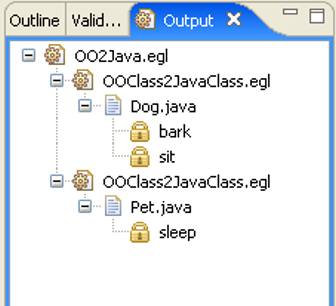
\includegraphics[scale=0.6]{images/TraceView}
  \end{center}
  \caption{Sample output from the traceability API.}
  \label{fig:traceability}
\end{figure}


\begin{lstlisting}[language=Java, basicstyle=\ttfamily\footnotesize, language=EGL, tabsize=2, flexiblecolumns=true, caption=Programmatically accessing the EGL traceability API (in Java)., label=lst:traceability]
	IEolExecutableModule module = 
	  new EglTemplateFactoryModuleAdapter(new EglTemplateFactory());
	
	boolean parsed = module.parse(new File("myTemplate.egl"));
	
	if (parsed && module.getParseProblems().isEmpty()) {
		module.execute();

		Template base = module.getContext().getBaseTemplate();
		
		// traverse the template hierachy
		// display data 
		
	} else {
		// error handling
	}
\end{lstlisting}